\section{Overview}
\label{sec:greybox-overview}

This section presents the target program structure, workflow, and intended use of \greyboxfuzz. We first describe the structure of a \zksnark application and introduce the terminology used throughout the paper in that context. We then explain why existing fuzzing approaches are insufficient for detecting \logicerror in \zksnark binary programs. Finally, we describe the workflow of \greyboxfuzz, along with its intended users and use cases.

\subsection{Structure of a \zksnark Program}
\label{subsec:greybox-structure_zkp}

\begin{figure}[ht]
  % \vspace*{6pt}
  \centering
  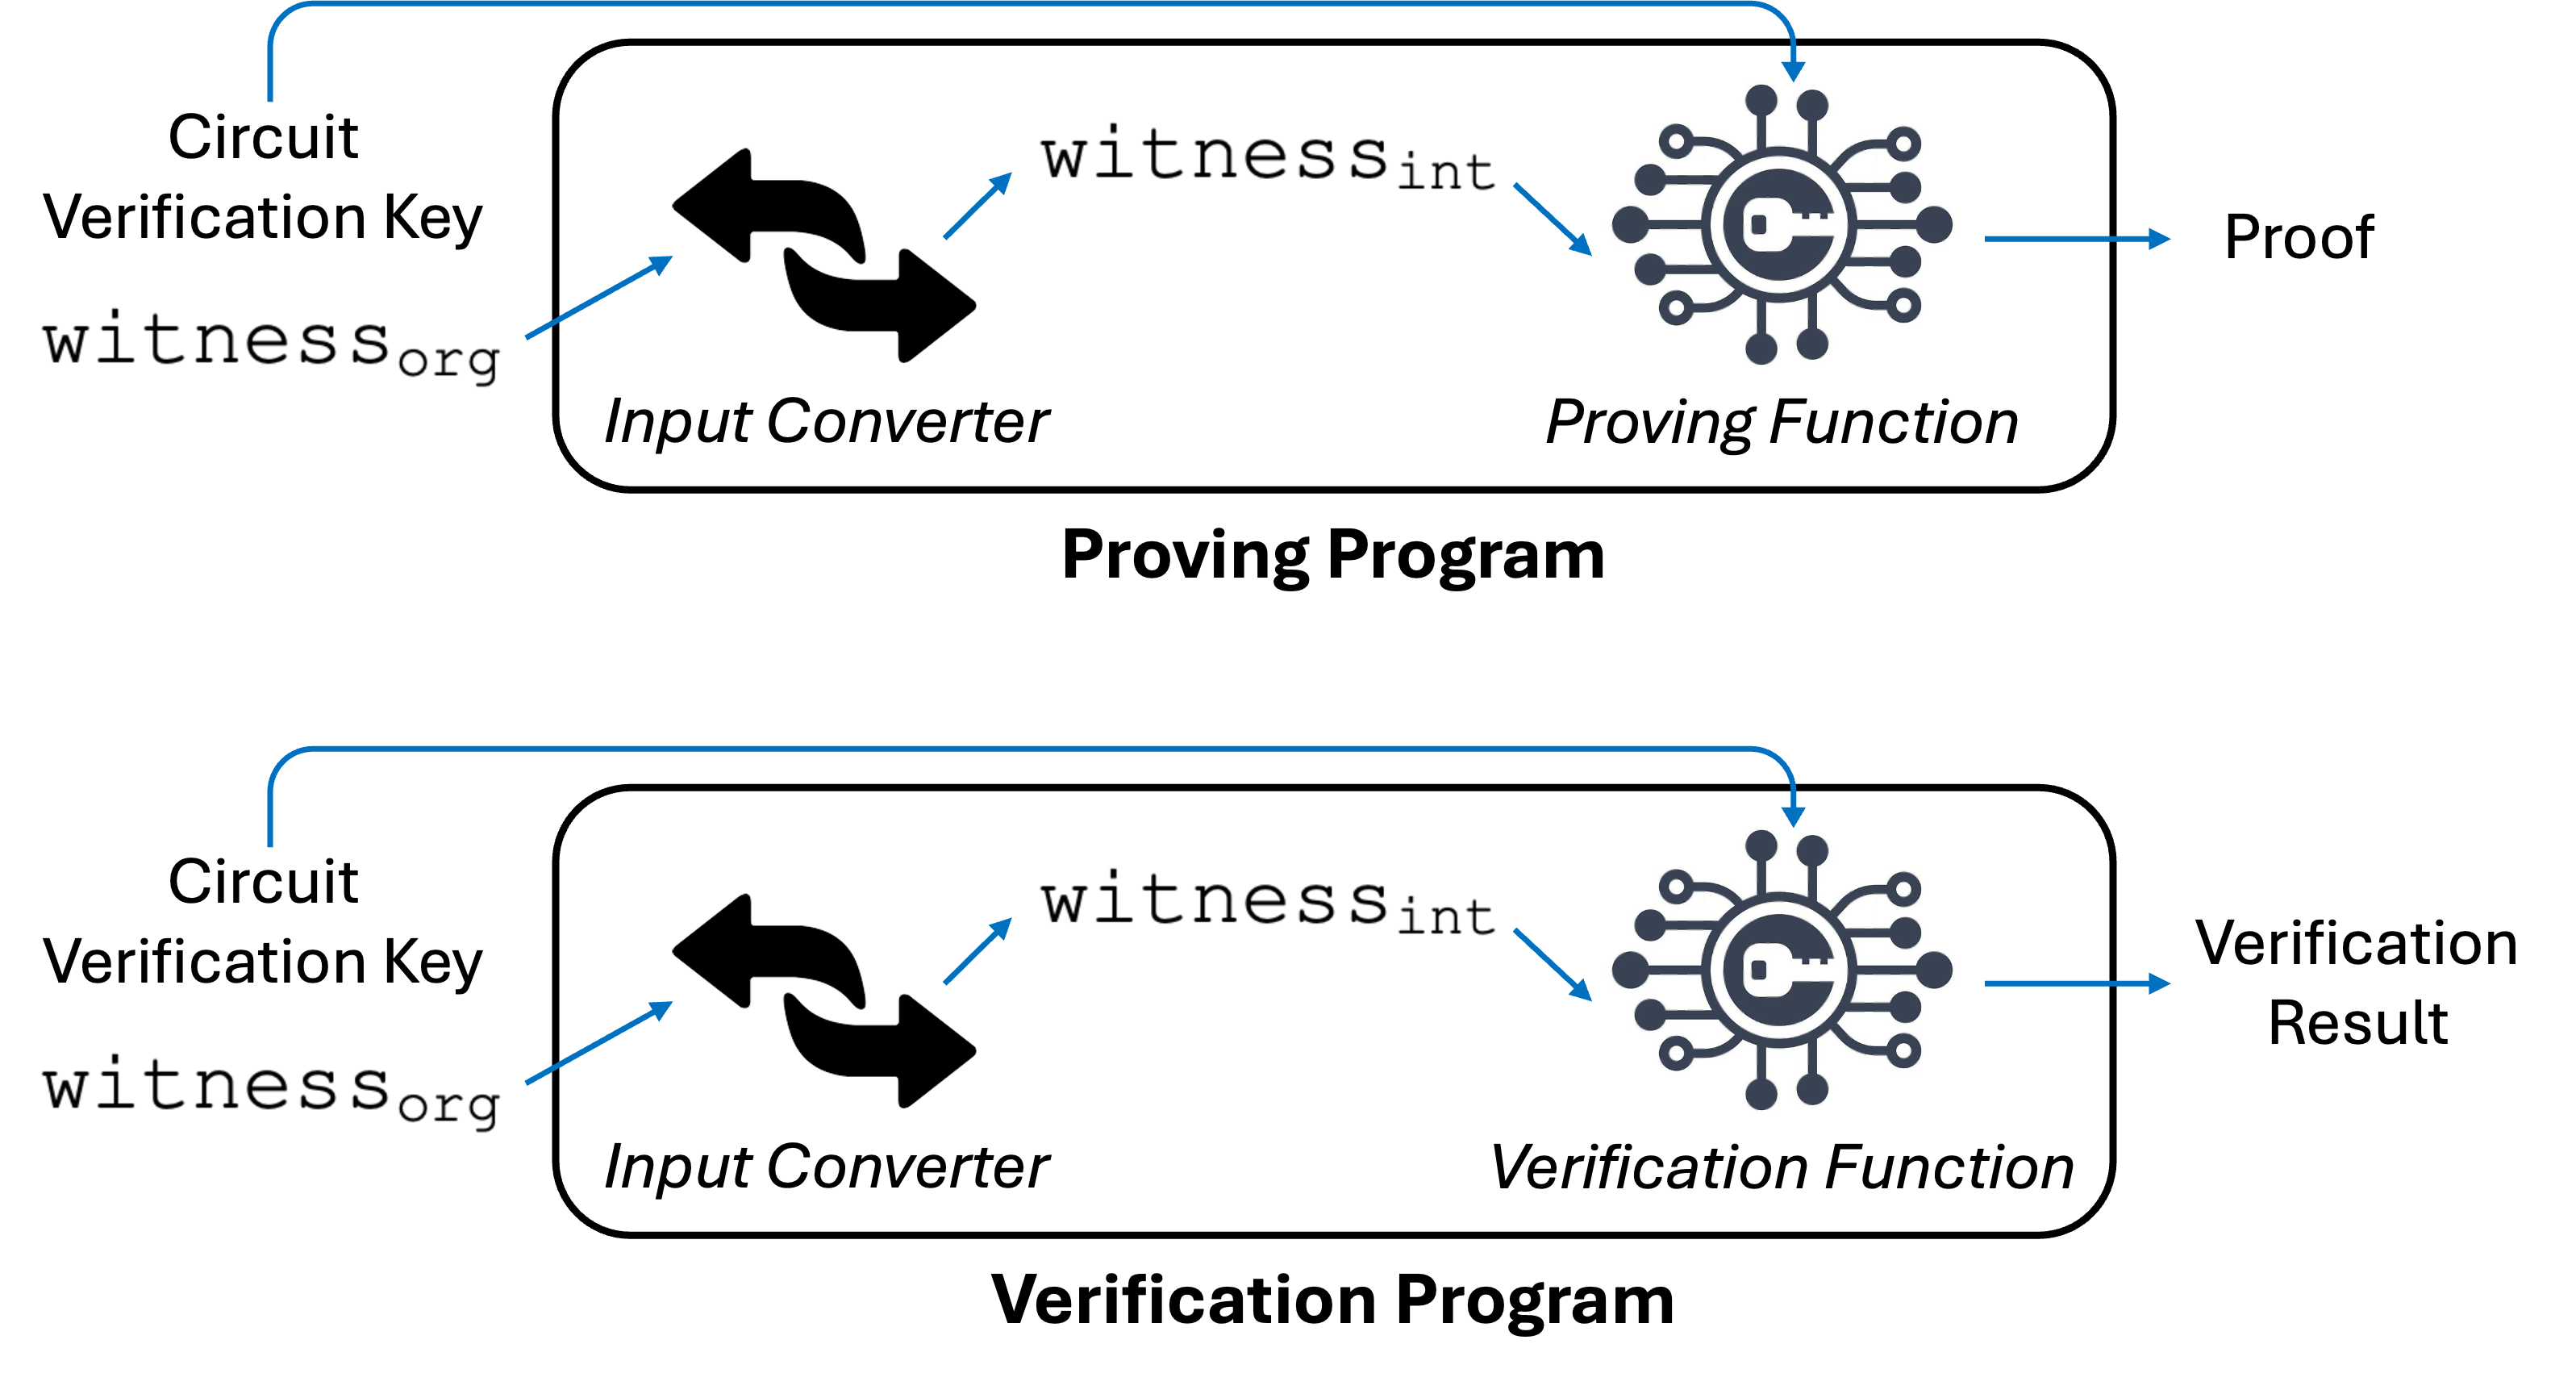
\includegraphics[width=0.5\textwidth,keepaspectratio]{./ch-greybox/figure/structure_zkp.png}
  \caption{Structure of a \zksnark program. }
  \label{fig:structure_zkp}
\end{figure}

A \zksnark application typically contains two complete programs: a prover-side program, denoted by \pprog, and a verifier-side program, denoted by \vprog. Each complete program contains both general program logic and a core cryptographic function. \autoref{fig:structure_zkp} illustrates this structure.

The prover-side program \pprog receives the original witness \witnessorg, a circuit representation such as a Rank-1 Constraint System (R1CS), and a proving key. The original witness contains both public and private values. Since the core proof-generation function \pfunc operates on the algebraic format required by the underlying proof system, \pprog first applies an \inputconvert step to transform \witnessorg into the internal witness representation \witnessint. This internal representation typically encodes values in forms suitable for proof computation, such as finite-field elements, ordered vectors, or other system-specific structures, rather than the original application-level format. For example, an application may provide a witness value as a decimal integer or a structured object, while the proof system requires that value to be represented as one or more finite-field elements in a fixed order. After this conversion, \pfunc uses \witnessint, the circuit, and the proving key to generate a proof.%, since the proof-generation algorithm operates over the field and group representations required by the underlying proof system rather than directly on application-level values.

The verifier-side program \vprog receives the proof, the public witness, and a verification key. The verifier does not receive the prover's private witness. However, the public witness still needs to be parsed and converted into the internal representation expected by the verification function \vfunc. Therefore, similar to \pprog, \vprog also contains an \inputconvert step for public witness. After conversion, \vfunc checks the proof with respect to the public witness and verification key, and outputs either accept or reject.

This structure creates several possible sources of \logicerror. An inconsistency may originate from the circuit, the prover-side \inputconvert, the proof-generation function, the verifier-side \inputconvert, or the verification function. Therefore, detecting that an error exists is not sufficient. A practical testing tool should also help locate which component is responsible for the error.

Depending on the specific proof system, a setup phase may also be required before \pprog and \vprog are executed. For example, many \zksnark protocols require a setup process to generate parameters such as proving key and verification key. These setup artifacts are treated as inputs to the corresponding prover and verifier programs.

In the remainder of this paper, we use the term \emph{software error} to refer to observable program failures, such as crashes, memory errors, assertion failures, or abnormal termination, and we use \logicerror{} to refer to cryptographically incorrect behavior that may not cause any runtime failure. We also distinguish between \programbranch, which handles general program functionality such as parsing, memory management, and input/output, and \cryptobranch, which performs cryptographic computation or directly influences cryptographic computation, such as proof generation, proof verification, finite-field arithmetic, elliptic-curve operations, constraint evaluation, and protocol-specific logic.

\subsection{Motivation for Grey-Box Fuzzing of \zksnark Programs}
\label{subsec:greybox-motivation_greybox}
General-purpose fuzzing tools are effective at detecting software errors in cryptographic programs. For example, fuzzers such as \afl can generate inputs that expose crashes, buffer overflows, null pointer dereferences, and other memory-safety issues. However, many serious errors in \zksnark implementations are \logicerror{}s rather than ordinary software errors. A \zksnark program may execute successfully but still produce an incorrect proof, accept an invalid proof, reject a valid proof, or enforce a statement different from the intended one. Since these errors may not cause crashes or abnormal termination, crash-oriented fuzzing alone cannot reliably detect them.

Differential fuzzing provides a more suitable foundation for detecting \logicerror because it checks whether the target implementation produces the expected cryptographic result rather than merely observing whether the program crashes. In principle, a fuzzer can compare the output of a target \zksnark program against the expected accept-or-reject result of the intended statement and report inconsistencies such as accepting an invalid witness or rejecting a valid one. This makes differential fuzzing a natural starting point for testing \zksnark correctness.

Among possible differential fuzzing designs, a grey-box approach is particularly suitable for real-world \zksnark applications. Unlike source code based approaches, grey-box fuzzing can be applied directly to deployed binary programs, which is important when source code is unavailable. At the same time, it can use internal information from the target \zksnark program to improve testing efficiency. In our setting, this is especially valuable because \zksnark applications follow structured cryptographic workflows that can benefit from protocol-aware guidance even in binary-only form.

The first major obstacle is input generation. General-purpose fuzzers mutate byte sequences without understanding the structure or meaning of cryptographic inputs. As a result, they often produce malformed witnesses, invalid field elements, incorrectly encoded group elements, or proof objects that are rejected before execution reaches the core cryptographic computation. Although such inputs may still be useful for testing parsers or input validation code, they are inefficient for finding logic errors in proof generation or verification. To reach deeper cryptographic computation, the fuzzer must generate inputs that preserve the expected format while still exploring valid, invalid, and boundary-case values.

The second obstacle is coverage guidance. General fuzzers usually reward any input that discovers a new execution path. In \zksnark software, however, many execution paths are unrelated to cryptographic correctness, such as file parsing, memory allocation, data-structure handling, and general input/output code \cite{wen2024practical, 0xparc_zk_bug_tracker}. Exploring these paths may increase overall coverage, but it does not necessarily improve the chance of detecting proof-related logic errors. A more effective strategy is to identify the branches that depend on cryptographic inputs and prioritize inputs that exercise those branches.

These challenges motivate the design of \greyboxfuzz. By combining differential fuzzing with structure-aware input generation and cryptographic-branch-focused coverage guidance, \greyboxfuzz improves the practicality and efficiency of testing binary-only \zksnark applications.


\subsection{Workflow}
\label{subsec:greybox-workflow}

\begin{figure*}[t]
  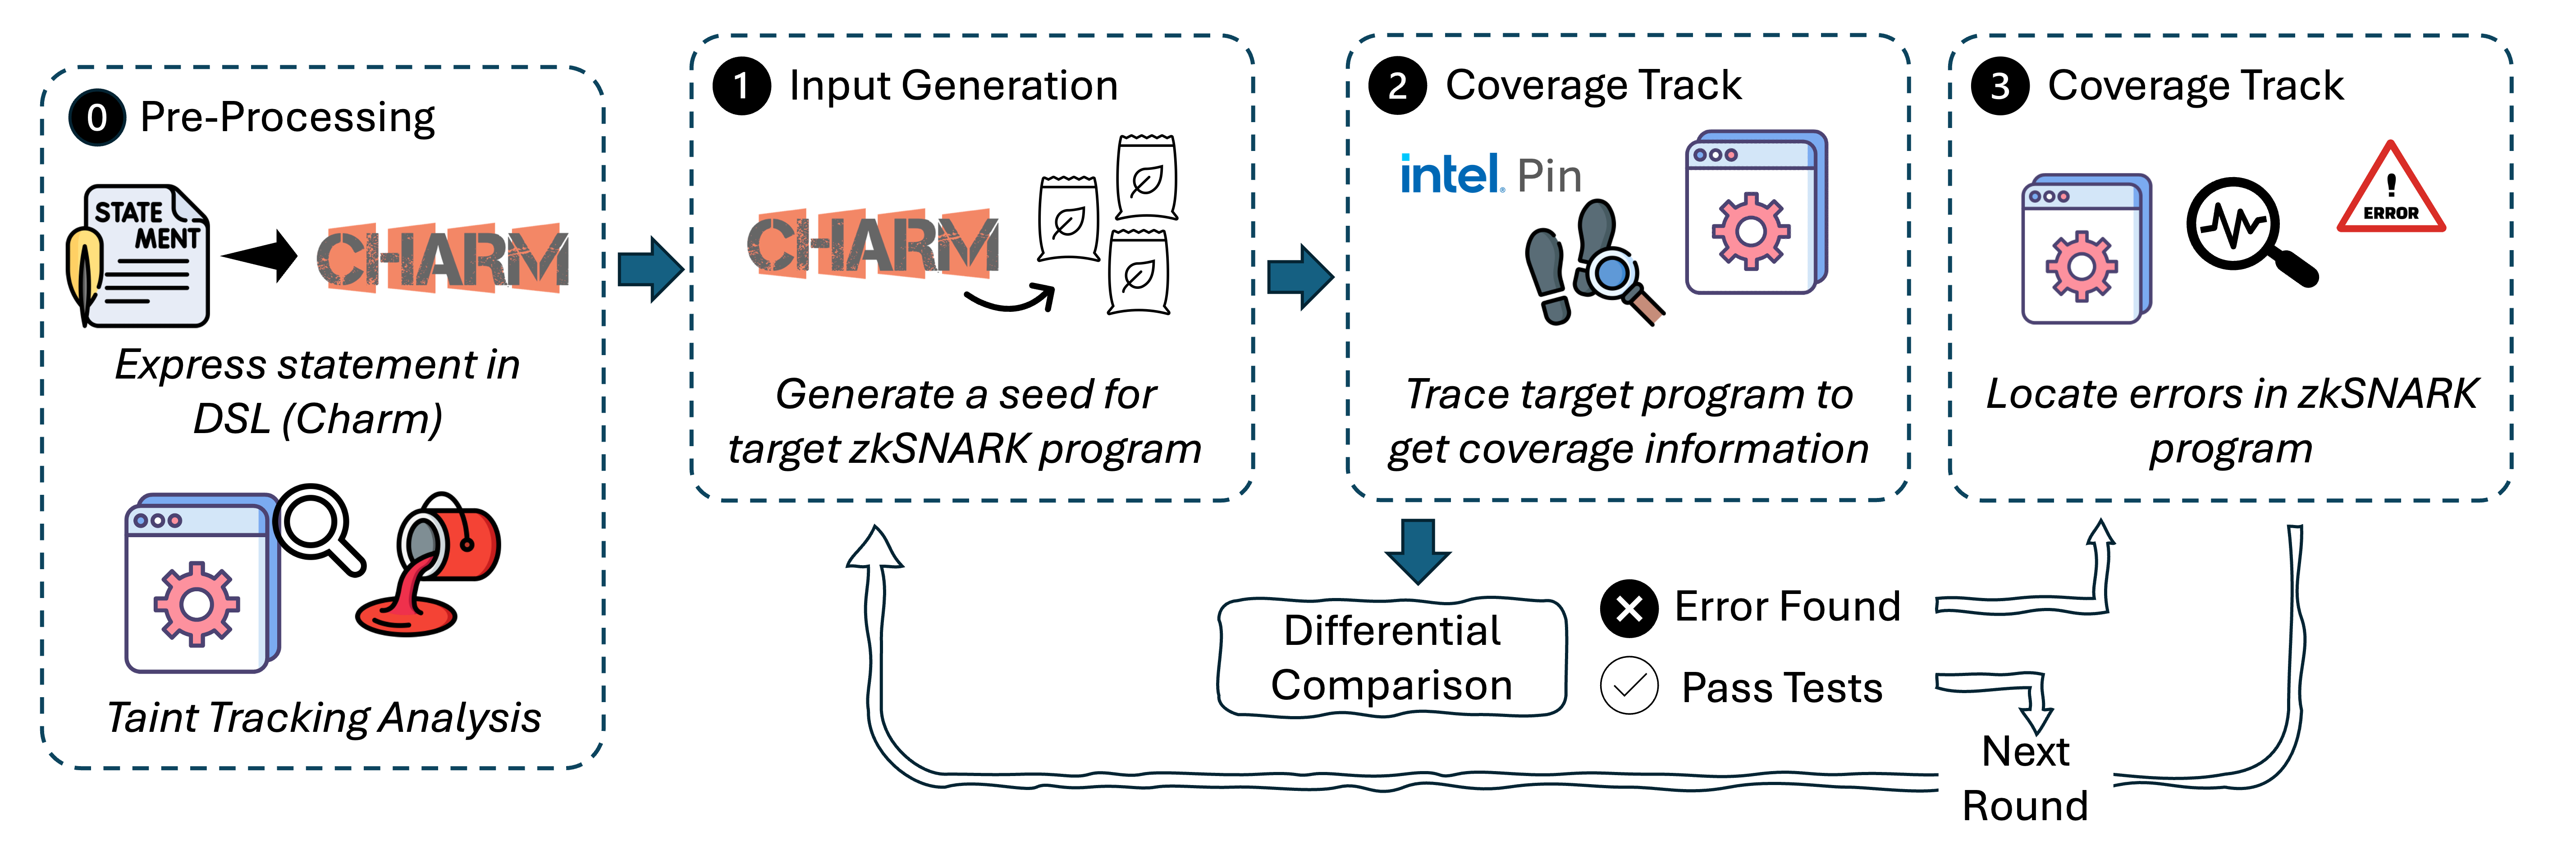
\includegraphics[width=\textwidth,keepaspectratio]{./ch-greybox/figure/overview.png}
  \caption{Overview of \greyboxfuzz.}
  \label{fig:overview}
\end{figure*}

\autoref{fig:overview} shows the workflow of \greyboxfuzz. To achieve the design goals and address the obstacles described in \autoref{subsec:greybox-motivation_greybox}, the workflow consists of five main components: differential test vector and ground truth for generating the expected result for a \zksnark program, preprocessing for investigating the target \zksnark program and obtaining additional information to improve fuzzing efficiency, input generation for producing suitable test inputs for effective fuzzing of \zksnark programs, coverage monitoring for tracking testing progress, and error localization as a new feature not provided by previous fuzzing tools.

\parhead{Differential ground truth}
For each generated seed, \greyboxfuzz executes the target \pprog and \vprog and compares the output with the expected result derived from the user-provided statement. In this process, the high-level cryptographic statement serves as the test vector and ground truth. Instead of requiring developers to implement a separate reference program for the entire \zksnark program, \greyboxfuzz evaluates the generated inputs against the statement to obtain the expected result and then compares that result with the output of the target binary program. If both results agree, the seed does not expose a \logicerror. If the target program accepts an input that should be rejected, rejects an input that should be accepted, or otherwise produces a result inconsistent with the statement, \greyboxfuzz reports a potential error.

\parhead{Preprocessing}
Before fuzzing begins, \greyboxfuzz performs a one-time analysis of the target binary programs. Since \greyboxfuzz targets binary-only \zksnark programs, it cannot rely on source-code instrumentation. Instead, it applies static taint tracking to identify \cryptobranch in the target binaries. These branches are the parts of the program that depend on \zksnark inputs, such as the witness, circuit, proving key, verification key, and proof. Identifying these branches allows \greyboxfuzz to distinguish security-relevant cryptographic computation from general program logic.

During preprocessing, \greyboxfuzz also identifies program locations needed by the error locator. These locations are used to separate the complete prover and verifier programs into smaller logical components, such as \inputconvert, proof generation, and proof verification. This enables \greyboxfuzz to provide more useful feedback when it detects an inconsistency and helps narrow the component most likely responsible for the error.

\parhead{Input generation}
After preprocessing, \greyboxfuzz generates and mutates input seeds for the target program. Unlike general-purpose fuzzers, \greyboxfuzz uses a structure-aware input formatter that understands the structure of the cryptographic statement. The user provides the intended statement in a domain-specific language, and \greyboxfuzz uses this statement to infer the expected input types and constraints. In our current implementation, we use Charm as the domain-specific language tool. The formatter extracts variable information from the statement written with Charm and uses it to guide both seed generation and mutation. It distinguishes among input structure, mathematical validity, and statement-level value validity. This design allows \greyboxfuzz to produce seeds that preserve the legal format expected by the target program while still exploring invalid, boundary-case, and security-relevant values.

\parhead{Coverage monitoring}
During execution, \greyboxfuzz records which binary instructions are visited by each seed. Because \greyboxfuzz focuses on \logicerror, it does not treat all new execution paths equally. Instead, it prioritizes seeds that visit new \cryptobranch. To support this strategy, \greyboxfuzz combines static taint tracking with dynamic tracing. Static taint tracking identifies instructions that belong to the cryptographic related branches, while dynamic tracing records whether generated seeds reach those cryptographic-related branches. Inputs that explore new \cryptobranch are prioritized, whereas inputs that only expand general programming coverage receive less attention. This prevents the fuzzer from spending excessive time exploring general parsing, input/output, or memory-management code when those paths do not affect the cryptographic result.

\parhead{Error localization}
When \greyboxfuzz detects an inconsistency, it invokes the error locator. A \zksnark program may fail because of an incorrect implementation in circuit, \inputconvert, proof-generation function \pfunc, or verification function \vfunc. The error locator therefore analyzes multiple intermediate components, including the circuit, converted witness values, proof-generation behavior, and verification behavior, to narrow the source of the error. Instead of only reporting that the target program failed, \greyboxfuzz attempts to identify whether the error is caused by the circuit, the prover-side \inputconvert, \pfunc, the verifier-side \inputconvert, or \vfunc. This feedback helps developers diagnose and fix \logicerror in binary-only \zksnark implementations.

\subsection{Users and Use Cases}
\label{subsec:greybox-users_use_cases}

\greyboxfuzz is designed for users who need to evaluate the correctness and security of a specific \zksnark application but may not have the ability to audit the entire implementation manually. This includes both prover-side and verifier-side users.

From the prover's perspective, the main concern is whether the program correctly proves the intended statement using the provided witness. A prover-side error may cause a valid witness to be converted incorrectly, a valid proof to fail, or the proof-generation process to enforce a statement different from the intended one.

From the verifier's perspective, the main concern is whether an invalid proof can be accepted. If a prover can generate a proof using values that do not satisfy the intended statement, then the verifier should not trust the proof in that setting. Such a result may indicate an error in the circuit, witness conversion, proof generation, verification, or the surrounding program logic.

To use \greyboxfuzz, the user provides the prover binary program, the verifier program, and the \zksnark statement written with Charm. \greyboxfuzz then generates test inputs, checks the target program against the statement, monitors cryptographic coverage, and reports both detected inconsistencies and their likely locations. This allows users to evaluate a specific proof application without requiring source-code access or a complete manual audit of the underlying \zksnark library.


